\section{Dean-Kawasaki Validation}\label{sec:dk_validation}

\subsection{Dean-Kawasaki Implementation}\label{sec:dk_implementation} 
We now present the Dean-Kawasaki problem considered, the finite difference scheme
used,
following \cite{cornalba2025multilevel}, and our MLMC 
implementation.
We consider the Dean-Kawasaki equation on a one dimensional torus
$\Omega=[0,2\pi)$ with periodic boundary conditions and final time $T>0$.
The particle number is denoted $N_p$. The density 
field $\rho$ evolves according to

\begin{align}
\frac{\partial \rho(t,x)}{\partial t}
&= \frac{1}{2}\,\frac{\partial^2 \rho(t,x)}{\partial x^2}
\;+\; N_p^{-1/2}\,\frac{\partial \!\left(\sqrt{\rho(t,x)}\,\xi(t,x)\right)}{\partial x},
&& (t,x)\in (0,T]\times [0, 2\pi),
\label{eq:dk_spde_problem}\\[4pt]
\rho(0,x)
&= Z_0\!\left(1+\frac{1}{\sqrt{2\pi}}
\,\exp\!\left(-\tfrac{1}{2}\,\sin^2\!\big(x-\tfrac{\pi}{2}\big)\right)\right),
&& x\in\Omega, \nonumber\\
\rho(t,0) &= \rho(t,2\pi), &&t \in [0,T], \nonumber
\end{align}
where $\xi$ is space-time white noise and $Z_0 \approx 
0.12$ is a normalisation constant.

We discretise $\Omega$ with a uniform grid of spacing 
$\Delta x, \Delta t$ and denote by $\rho_j^n$ the approximation
to $\rho(t_n, x_j)$ at time $t_n = n \Delta t$ and position $x_j = 
\Delta x$.

\begin{align}
\rho_j^{\,n+1}
&= \rho_j^{\,n}
\;+\; \tfrac{\lambda}{2}\,\bigl(\rho_{j+1}^{\,n}-2\rho_j^{\,n}+\rho_{j-1}^{\,n}\bigr)
\;+\; \tfrac{1}{\sqrt{N_p}}\,
\frac{F_{j+1}^{\,n}-F_{j-1}^{\,n}}{2\Delta x}, \label{eq:dk_fd}\\[4pt]
F_j^n &:= \sqrt{[\rho_j^n]_+}\,\Delta W_j^n, \qquad
\Delta W_j^n \overset{\text{i.i.d.}}{\sim} \mathcal{N}\!\left(0,\ \tfrac{\Delta t}{\Delta x}\right).
\nonumber
\end{align}

Our quantity of interest is the expected squared mean field fluctuations
in the $\sin(x)$ mode at final time $T$, namely

\begin{equation}\label{eq:dk_qoi}
P = \mathbb{E}\!\left[\,N_p \left(\int_0^{2\pi} 
\big(\rho(T,x)-\bar{\rho}(T,x)\big)\,\sin(x)\,\mathrm{d}x\right)^{\!2}\right],
\end{equation}
where $\bar\rho$ denotes the deterministic mean-field solution.

In the discrete setting, we approximate this by
\begin{equation}
P \;=\; N_p \left( \big(\boldsymbol{\rho}^N - \boldsymbol{\bar\rho}^N,\ 
\sin(x_h)\big)_h \right)^{\!2},
\end{equation}

To compute $P$, we update in parallel the 
deterministic mean-field 
solution $\bar\rho$ via an explicit finite difference scheme for the 
heat equation.

Our MLMC implementation is performed in the same manner as that 
used for the Stochastic Heat Equation,
We set $\Delta x_\ell = 2 \pi / 2^{l + 1}$, $\lambda = \frac{1}{4}$
and set $\Delta t = \lambda (\Delta x)^2$, ensuring stability 
\cite{cornalba2025multilevel}.
For our quantity of interest, we take $T=0.25$.

For coupling methods, we implement the NN and CC methods outlined in 
Section \ref{sec:she_scheme_mlmc_imp}. The NN method is 
used to replicate the results from Cornalba and Fischer \cite{cornalba2025multilevel}.
We then compare this with the proposed CC method to assess 
whether the symmetric coupling provides any tangible performance 
improvements.

\subsection{Dean-Kawasaki Validation}\label{sec:dk_validation}

We now verify that our implementation converges. We obtained an estimate of the true 
value of \eqref{eq:dk_qoi} via MC simulation, and now verify convergence 
of our implementation across a range of accuracies, 
$\varepsilon \in \{0.001, 0.005, 0.01, 0.05\}$. We also again 
analyse variance and error decay. The results are summarised in Table 
\ref{tab:dk_rates} and Figures \ref{fig:dk_validation_combined},

\begin{table}[htbp]
    \centering
    \begin{tabular}{|l|c|c|r|}
        \hline
        \textbf{Coupling Method} & \textbf{$\alpha$} & \textbf{$\beta$} & \textbf{$\gamma$} \\
        \hline
        Nearest Neighbour & 2.11 & 1.95 & 3.0\\
        Central Coupling & 1.95 & 1.95 & 2.98 \\
        \hline
    \end{tabular}
    \caption{Empirically estimated rates for the DK QoI.}
    \label{tab:dk_rates}
\end{table}

\begin{figure}[htbp]
    \centering
    \begin{subfigure}{\textwidth}
        \centering
        \begin{subfigure}[b]{0.48\textwidth}
            \centering
            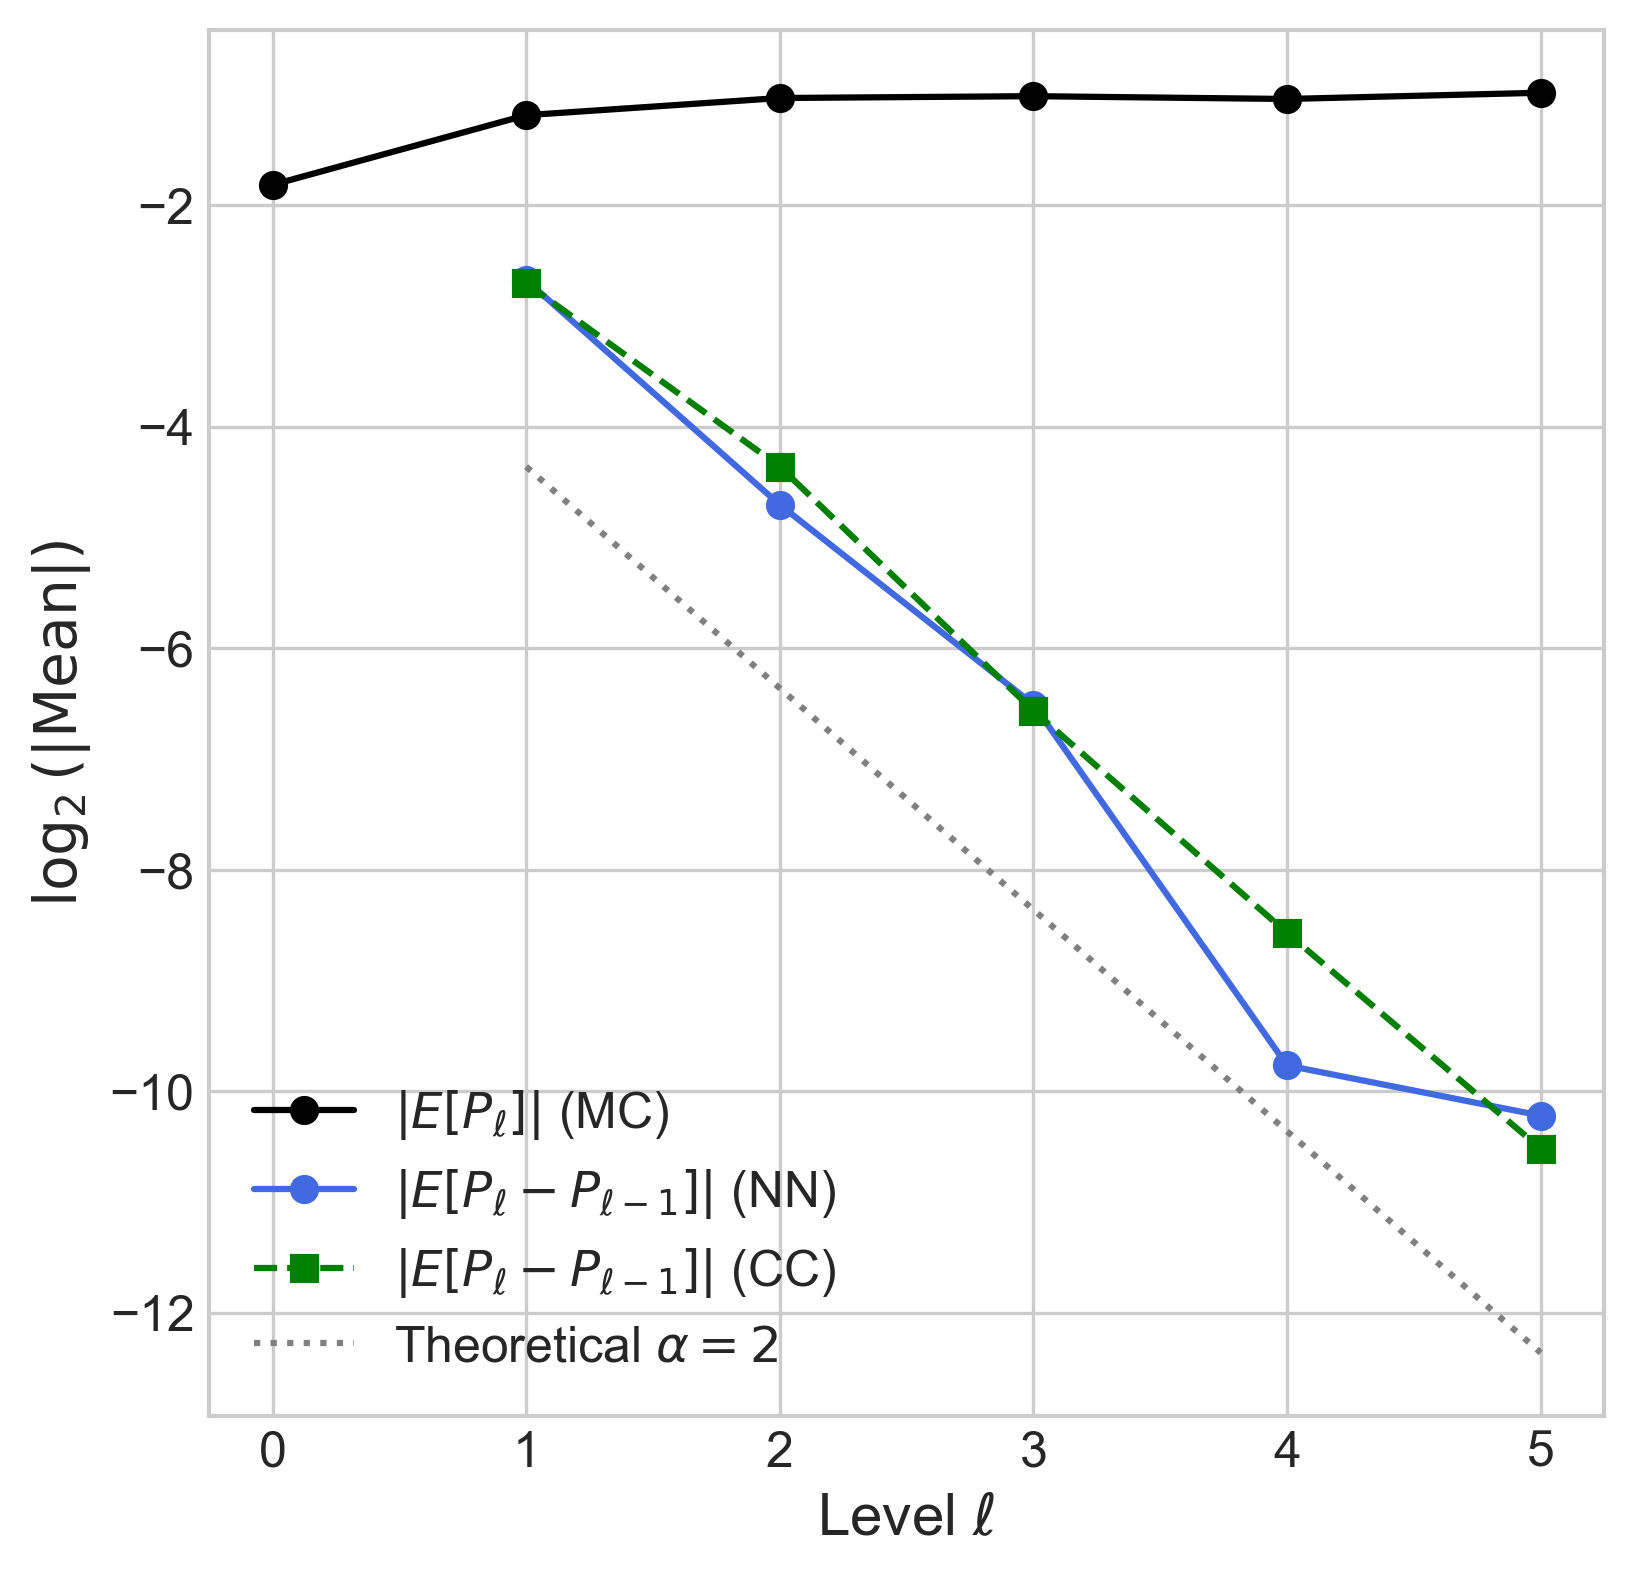
\includegraphics[width=\linewidth]{graphics/dk_err_decay.png}
            \caption{Weak error decay ($\alpha$).}
            \label{fig:dk_error_decay}
        \end{subfigure}
        \hfill
        \begin{subfigure}[b]{0.48\textwidth}
            \centering
            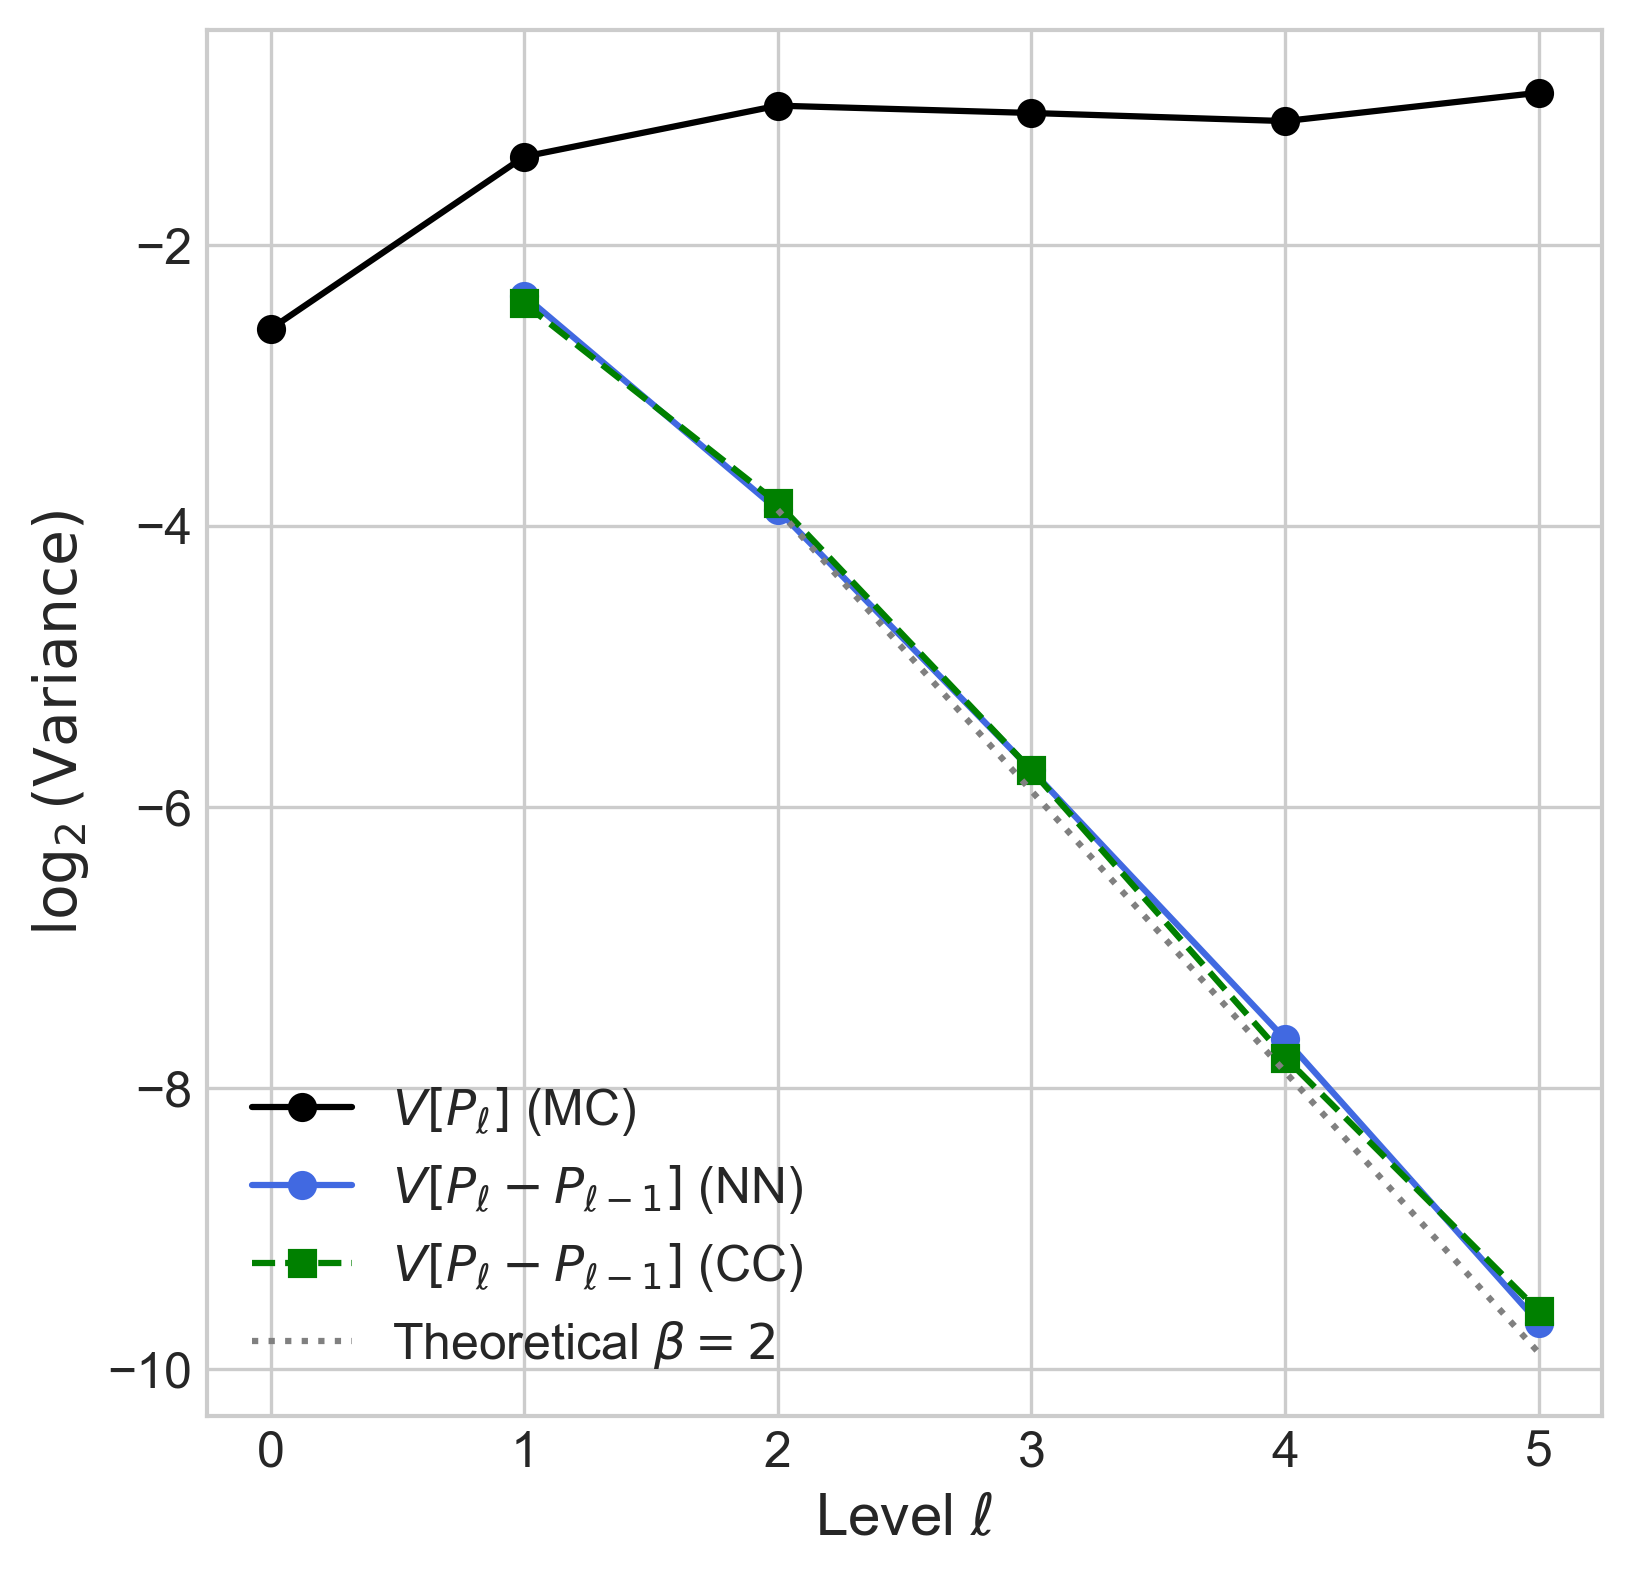
\includegraphics[width=\linewidth]{graphics/dk_var_decay.png}
            \caption{Variance decay ($\beta$).}
            \label{fig:dk_variance_decay}
        \end{subfigure}
    \end{subfigure}
    \vspace{1cm}
    \begin{subfigure}{\textwidth}
        \centering
        \begin{subfigure}[b]{\textwidth}
            \centering
            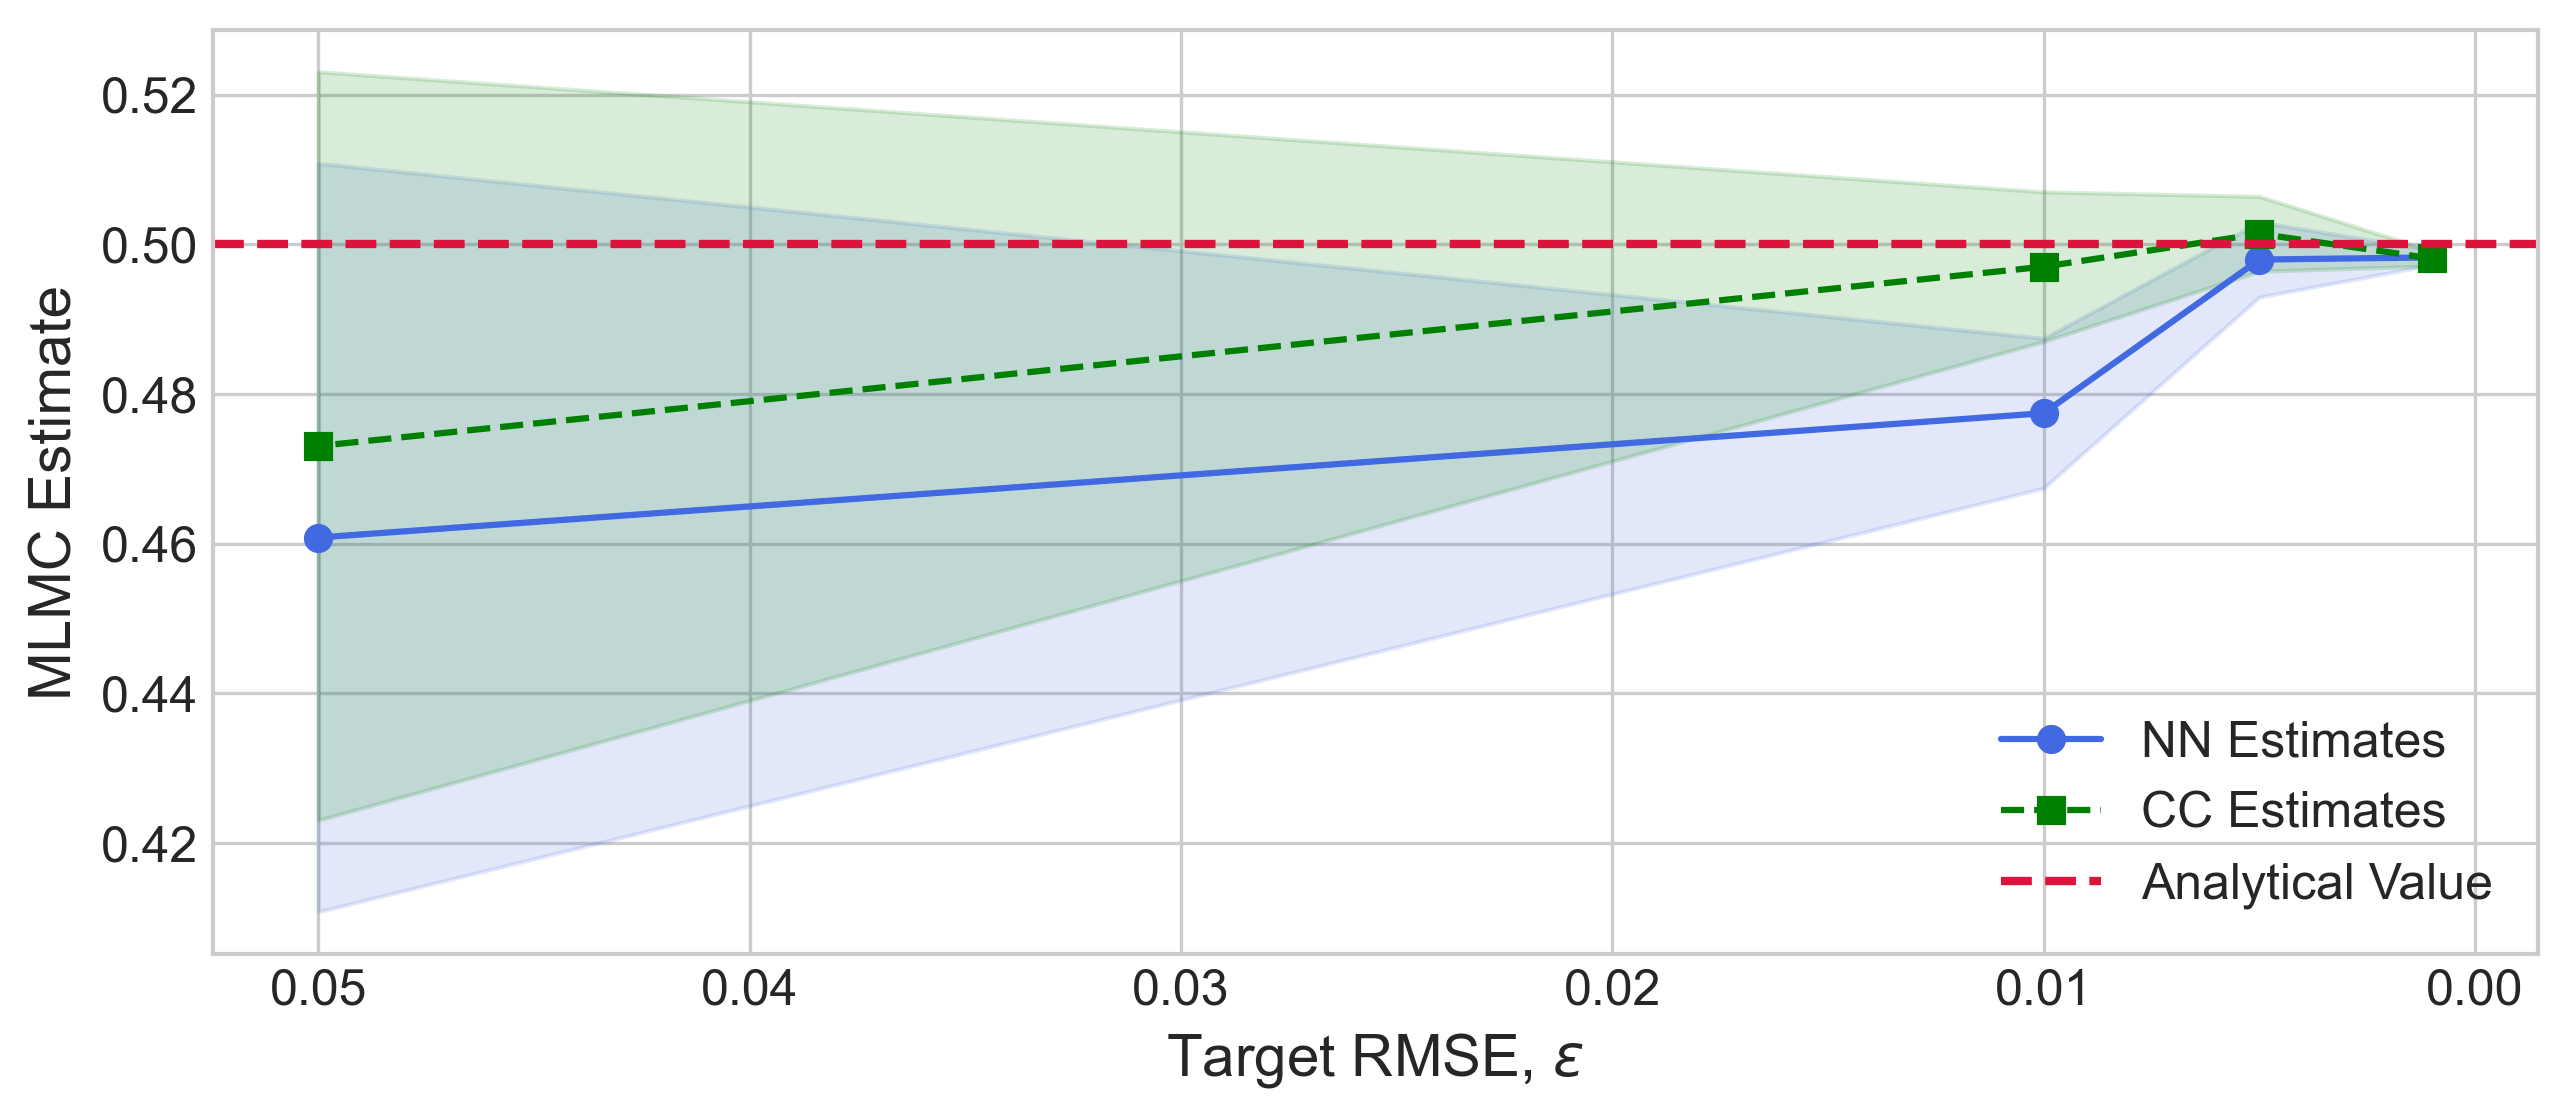
\includegraphics[width=0.7\linewidth]{graphics/dk_conv.png}
            \caption{Final MLMC estimate vs. target RMSE ($\varepsilon$).}
            \label{fig:dk_conv_vs_eps}
        \end{subfigure}
        \vspace{0.5cm}
        \begin{subfigure}[b]{\textwidth}
            \centering
            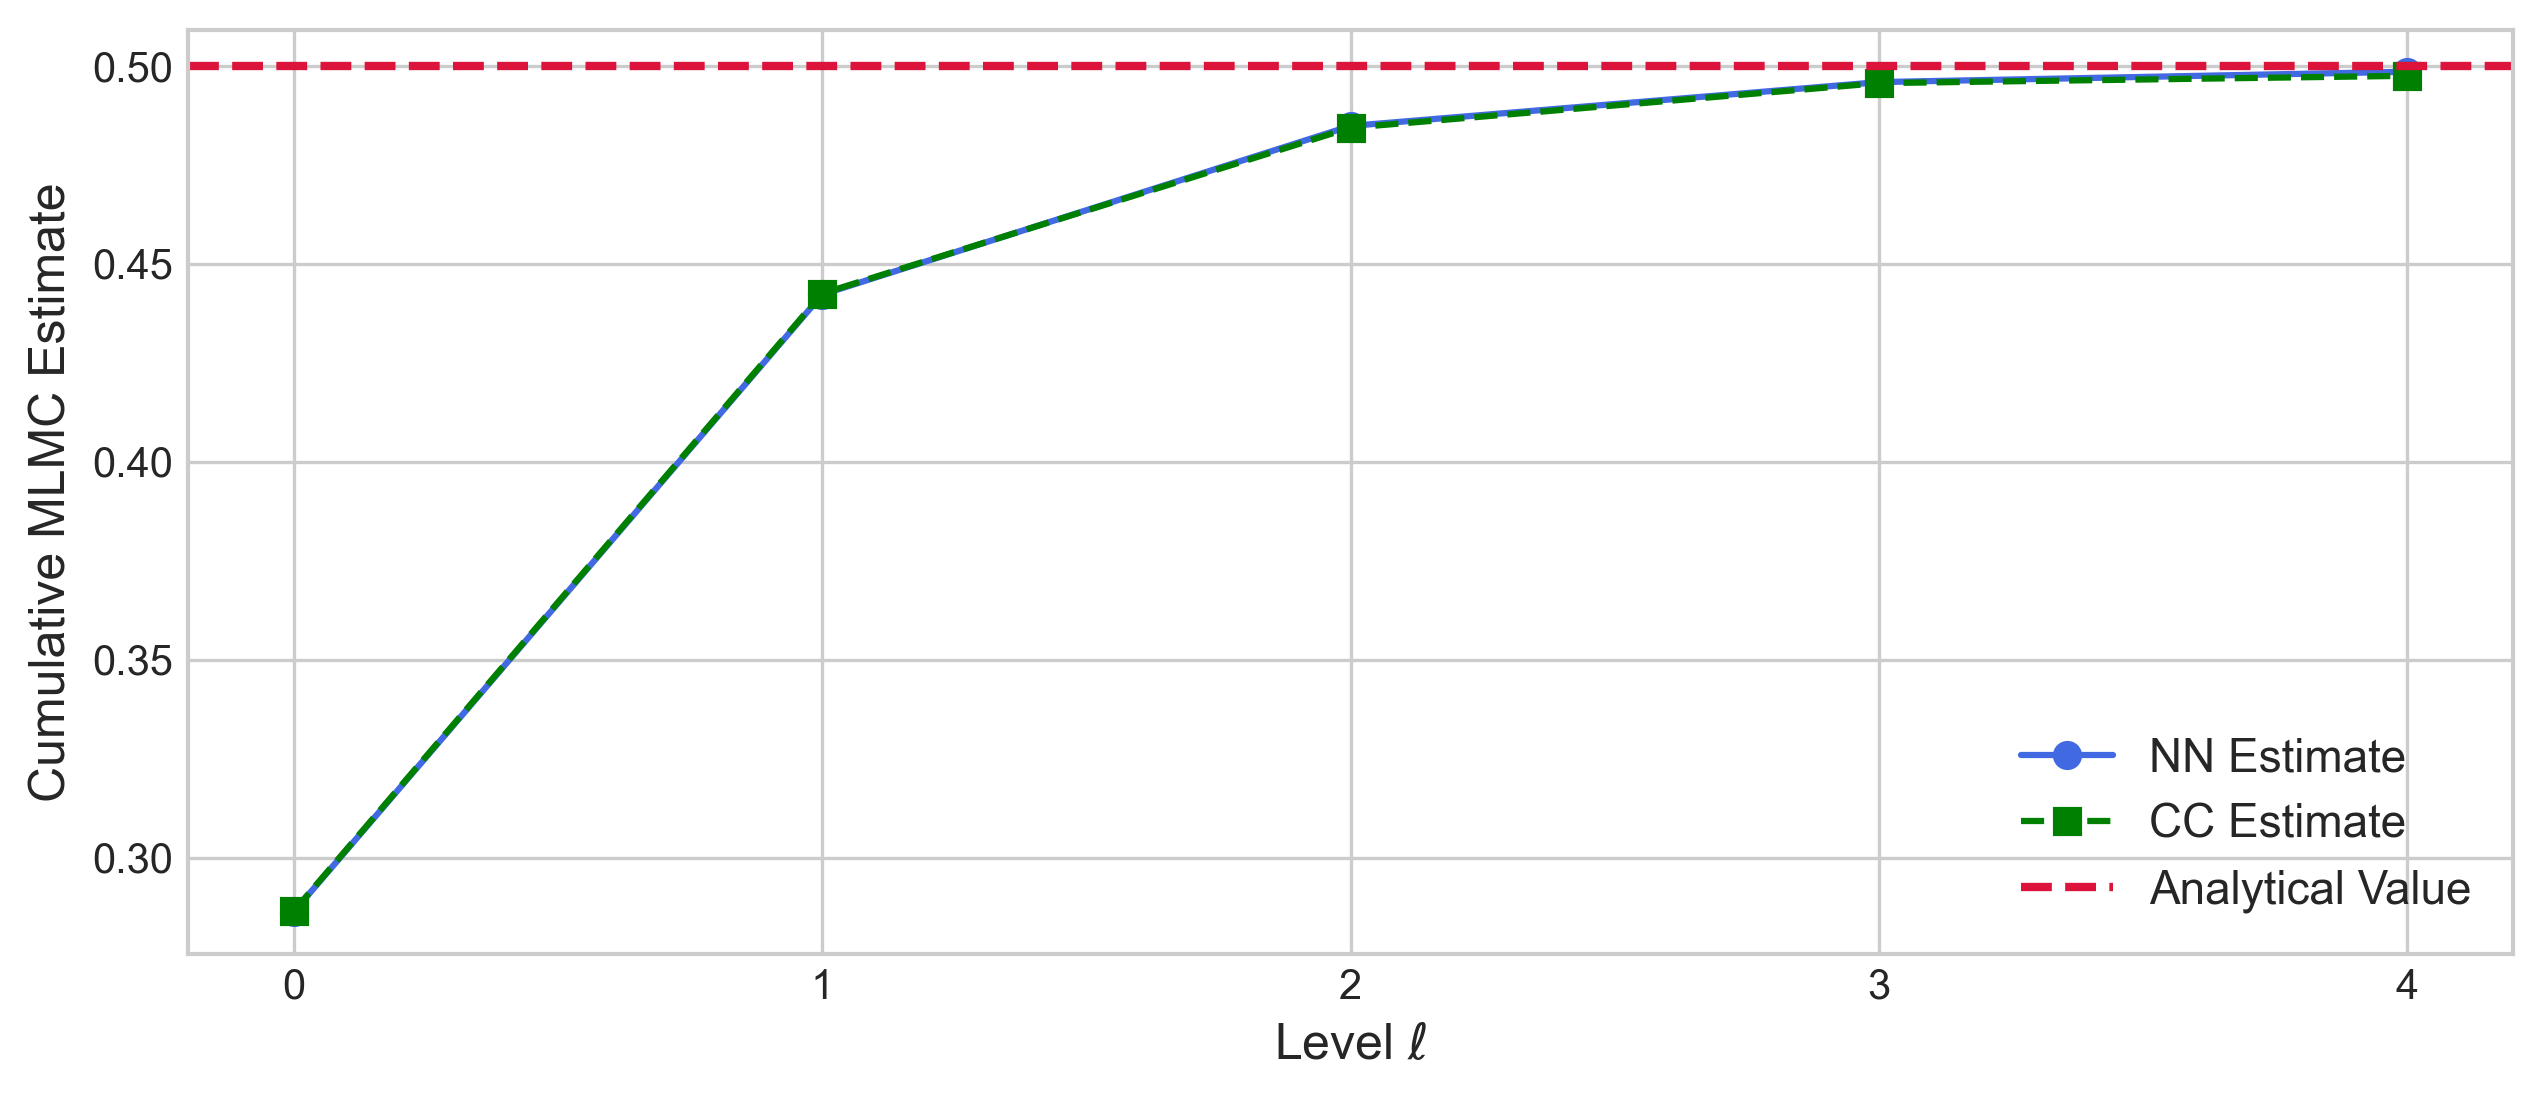
\includegraphics[width=0.7\linewidth]{graphics/dk_cumconv.png}
            \caption{Cumulative estimate vs. level ($\ell$) for $\varepsilon=0.001$.}
            \label{fig:dk_cumulative_conv}
        \end{subfigure}
    \end{subfigure}
    \caption{Validation and convergence plots for the MLMC implementation for the Dean-Kawasaki equation.}
    \label{fig:dk_validation_combined}
\end{figure}


The rates for the DK problem match those observed for the SHE. 
$\alpha \approx 2$ and $\beta \approx 2$ for both the 
CC and NN couplings, illustrated in Figures 
\ref{fig:dk_error_decay} and \ref{fig:dk_variance_decay}, and the 
expected $\gamma = 3$ for this scheme. Obtaining 
$\beta = 2$ aligns with the results found by Cornalba and Fischer 
for their NN coupling \cite{cornalba2025multilevel}, and again
we observe that the CC method behaves similarly to the NN.

Figure \ref{fig:dk_conv_vs_eps} shows that both coupling methods 
converge towards the analytic value of 
QoI across all RMSE tolerances. The cumulative convergence plot, 
Figure \ref{fig:dk_cumulative_conv}, demonstrates the 
standard behaviour of the MLMC estimator for both, and we again
observe equivalence between the two methods at the highest accuracy.



